\documentclass[11pt]{article}
\usepackage[utf8]{inputenc}
\usepackage{graphicx}
\usepackage{listings}
\usepackage{color}
\usepackage{float}
\usepackage[margin=1in]{geometry}
\usepackage{multirow}
\usepackage{multicol}
\usepackage{todonotes}
\usepackage[toc,page]{appendix}
\usepackage[square,numbers]{natbib}
\usepackage[utf8]{inputenc} % Required for inputting international characters
\usepackage[T1]{fontenc} % Output font encoding for international characters
% \usepackage{mathpazo} % Palatino font

\graphicspath{}

\usepackage{fancyvrb}

\usepackage{markdown}



\newtheorem{theorem}{RQ}

\lstdefinestyle{leftCode}{
  belowcaptionskip=1\baselineskip,
  breaklines=true,
  frame=L,
  xleftmargin=\parindent,
  showstringspaces=false,
  basicstyle=\footnotesize\ttfamily
}


\begin{document}

%----------------------------------------------------------------------------------------
%	TITLE PAGE
%----------------------------------------------------------------------------------------

\begin{titlepage} % Suppresses displaying the page number on the title page and the subsequent page counts as page 1
	\newcommand{\HRule}{\rule{\linewidth}{0.5mm}} % Defines a new command for horizontal lines, change thickness here
	
	\center % Centre everything on the page
	
	%------------------------------------------------
	%	Headings
	%------------------------------------------------
	
	\textsc{\LARGE University of Birmingham}\\[1.5cm] % Main heading such as the name of your university/college
	
	\textsc{\Large Department of Computer Science}\\[0.5cm] % Major heading such as course name
	
	\textsc{\large Dissertation for BSc. Mathematics and Computer Science}\\[0.5cm] % Minor heading such as course title
	
	%------------------------------------------------
	%	Title
	%------------------------------------------------
	
	\HRule\\[0.4cm]
	
	{\huge\bfseries Semantic Analysis of Text}\\[0.4cm] % Title of your document
	
	\HRule\\[1.5cm]
	
	%------------------------------------------------
	%	Author(s)
	%------------------------------------------------
	
	\begin{minipage}{0.4\textwidth}
		\begin{flushleft}
			\large
			\textit{Author}\\
			Tamara \textsc{Herbert} \\
			1557437% Your name
		\end{flushleft}
	\end{minipage}
	~
	\begin{minipage}{0.4\textwidth}
		\begin{flushright}
			\large
			\textit{Supervisor}\\
			Leandro \textsc{Minku} % Supervisor's name
		\end{flushright}
	\end{minipage}
	
	%------------------------------------------------
	%	Date
	%------------------------------------------------
	
	\vfill\vfill\vfill % Position the date 3/4 down the remaining page
	
	{\large April  2019} % Date, change the \today to a set date if you want to be precise
	
	%------------------------------------------------
	%	Logo
	%------------------------------------------------
	
	%\vfill\vfill
	
\includegraphics[width=0.2\textwidth]{litImgs/birmingham.png}\\[1cm] % Include a department/university logo - this will require the graphicx package
	 
	%----------------------------------------------------------------------------------------
	
	\vfill % Push the date up 1/4 of the remaining page
	
\end{titlepage}

%-----------------
\setcounter{tocdepth}{1}
\tableofcontents

\pagebreak
\section{Abstract}

The semantic analysis investigation produced by this project explores structures in which emotions can be represented in a computable format, primarily using a Valence-Arousal-Dominance structure, and optimising sentiment prediction tools using lexicon-based and machine learning methods. Existing semantic analysis tools usually only classify whether input text is positive or negative, and this project aims to explore other ways text can be classified.
Natural Language Processing tools are applied to text-based datasets, and various investigations are carried out to explore the best way to utilise the data for a prediction tool.

This project produces a machine learning model that takes an input sentence and returns Positive/Neutral/Negative classes for the Valence, Arousal and Dominance for the emotion behind the sentence. This model is then applied to a web application that uses this returned data to relate the text to music. 

The findings set out by this project imply that using a more complex structure to represent emotion can lead to a better understanding of input text, and shows that we can apply existing sentiment prediction methods to this structure to obtain an effective model.
\\
\textit{Keywords: Semantic Analysis, Machine Learning, Emotion Prediction, Text Analysis}
\pagebreak

\section{Introduction}

Analysing the emotions behind a piece of text is not always an easy problem even for human readers, and trying to compute this is much harder.

Sentiment analysis of text is a branch of Natural Language Processing where analysis is used to extract and identify subjective information from input data. This style of analytics has wide applications, primarily in marketing and customer service industries where materials such as social media and survey responses are utilised to provide intelligent information about a target market. 

Many sentiment analysis tools that already exist predict whether input text is positive or negative, but very few attempt to obtain more detail about the more complex mood behind it. Understanding something as subjective as an emotion cannot always be put into these discrete binary classes, and as such, exploring whether an emotion can be represented by more than just this one dimension could hold significant value. Applications for establishing a more detailed emotion behind a text could be working out whether a customer who has a complaint about a product is angry or just disappointed, so that appropriate reimbursement can be suggested.

Some existing projects look at how positive a piece of text is in more detail, sometimes ranking sentences on a scale between 1 and 10 but just an emotion over this single dimension is limiting, and exploring whether there is a better way to represent sentiment than this is an interesting topic.
Extensive research has gone into producing sentiment analysis models over a positive-negative dimension with a high level of prediction accuracy, and using the results of these investigations to apply to a more complex emotive prediction model is something that this project aims to examine.

We can formalise this into two main research questions that will be investigated as part of this project:

\subsection{Research Questions}


\begin{itemize}
    \item   \begin{theorem} 
                \label{RQ1}
                \textnormal{How can textual sentiment prediction be optimised?}
            \end{theorem}   
    \item   \begin{theorem} 
                \label{RQ2}
                \textnormal{Is using more than 1 dimension to classify emotions useful?}
            \end{theorem} 
\end{itemize}

After analysis of existing work and exploring what data is available, we can refine these questions further. 

\pagebreak


\section{Sentiment Representation Structures}

\subsection{Ekman's Six Basic Emotions}

There is no universally accepted model for representing sentiments, but a standard for classifying emotions in a categorical model is using Ekmans six basic emotions \cite{Ekman}. These are identified as Anger, Disgust, Fear, Happiness, Sadness and Surprise. Since there are only six discrete classes in which emotions can be placed, this can be argued to be very subjective when classifying \cite{emoBank}, but are very useful in portraying a general result back to user rather than numeric values. Other ways of representing emotion in discrete classes exist, such as Izards 12 categories, but they are not as popular as Ekman's representation and have less literature available \cite{izard1993stability} .

\subsection{Valence}
A very common way to classify phrases and sentences in sentiment analysis is to analyse the Valence of the text, as already briefly discussed \cite{frijda1986emotions}.

The Valence of a piece of text is how positive or negative is perceived to be, usually rated on a scale between 0 and 1, with 0 being negative.
Using Valence in a machine learning context is very useful, since many textual datasets exist that are already split into how positive a piece of text is, such as product or movie reviews which are frequently accompanied by a star rating. There is plenty of previous projects that use this as a way to represent emotion, taking in input text and outputting a Valence value usually on a numeric scale, so this is a good base to structure a more complex model on.

\subsection{Valence Arousal Dominance Structure}

The Valence-Arousal-Dominance (VAD) structure provides a 3D representation for emotions, with each variable being defined as follows \cite{VAD}:
\begin{itemize}
    \item Valence- How positive or negative the statement is (as before).
    \item Arousal- Degree of calmness or excitement, the energy of the statement. 
    \item Dominance- Degree of control over a situation.
\end{itemize}

This structure provides the extra information about an emotion that is needed for a more in depth analysis of text, so will be used as the scale to analyse input text with for this project.

Using VAD values allows for easy representation into the Ekman six basic emotions as well, using a standard for translating between them as shown in Table \ref{ekmansTable}.


\begin{table}[ht]
\caption{Ekmans emotions mapped to VAD values \cite{VADMapping}, with values ranging from 0 to 5}
\centering
\begin{tabular}{ |c|c|c|c|c|c|c| } 
 \hline
  & Anger & Disgust & Fear & Happiness & Sadness & Surprise \\ 
 \hline                        
 Valence & 1.23 & 1 & 0.9 & 4.53 & 0.93 & 3.5\\ 
 Arousal & 3.98 & 3.38 & 4 & 3.78 & 1.83 & 4.18\\ 
 Dominance & 3.13 & 2.78 & 1.43 & 3.65 & 1.68 & 2.18\\ 
 \hline
\end{tabular}
\label{ekmansTable}
\end{table}
\pagebreak
\section{Datasets}

There are two suitable datasets for this task which rank text using a VAD structure.

\subsection{Bag-of-Words}

The bag-of-words dataset contains 14,000 English words, each with a specific VAD value assigned \cite{wordsData}. Building a prediction model with this dataset would lose any context in which the words are in within a sentence as they would be treated each as separate entities, so is not ideal for a prediction task, but using it to create a lexicon-based bag of words style model will be investigated.

\begin{figure}[h]
\centering
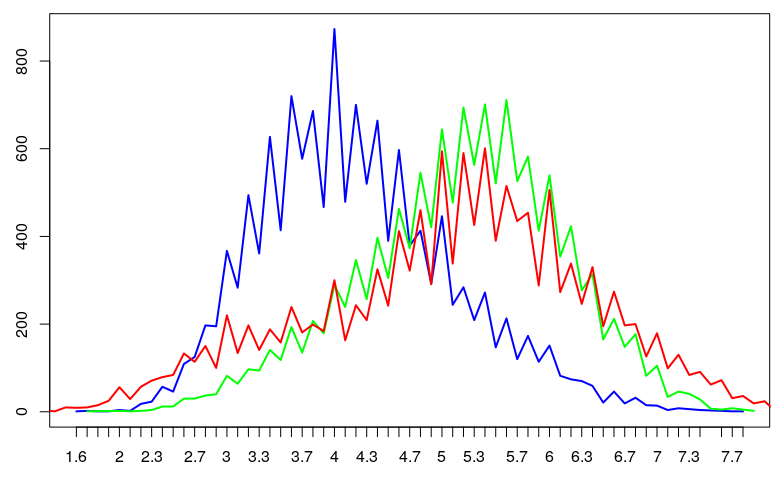
\includegraphics[scale=0.4]{graphs/lexiconDist.png}
\caption{Frequency of words over each dimension in bag-of-words dataset R: Valence, B: Arousal, G: Dominance. The dataset ranks the words on a scale between 0 and 10, which is adjusted for use with the EmoBank dataset}
\label{lexiconGraph}
\end{figure}

As we can see from Figure \ref{lexiconGraph} there is a bias in the data for each dimension, and the average value for the Arousal dimension is noticeably lower than the other two. Whether this affects the suitability of this dataset for use in building a prediction model will be explored further.

\subsection{EmoBank}
This dataset is the most important one for this project, as it contains 10,000 English sentences covering multiple genres, all annotated with their own VAD values \cite{emoBank}.

This dataset contains values for each sample sentence from both the writer and the reader of the text, but due to the findings in the paper accompanying it \cite{emoBank}, only the values given by the reader will be used, as it concluded that this perspective has higher emotionality and therefore they should be easier to build a more accurate model with.

Many existing sentiment analysis tools train over very large datasets, scraping information from things such as movie reviews \cite{socher2013recursive} or from Tweets \cite{towardsDS}, and so usually have above 100,000 samples to train from. In this case, the EmoBank dataset only contains 10,000 sentences, and whether this is a setback will have to be taken into account. These larger datasets could not be used in this case since they are not annotated in a way that allows a more complex emotion to be calculated, since they are usually only scored by their Valence values. 

We can see from Figure \ref{dist:vad} that most of the EmoBank data lies in the middle of the dataset, meaning that there is an imbalance in data. This can cause issues for building a prediction model from, as many prediction models will overfit on the majority class or range of values, predicting the most likely values every time. Dealing with this to be able to use the Emobank dataset in the most effective way will also be explored further.

\begin{figure}[h]
\centering
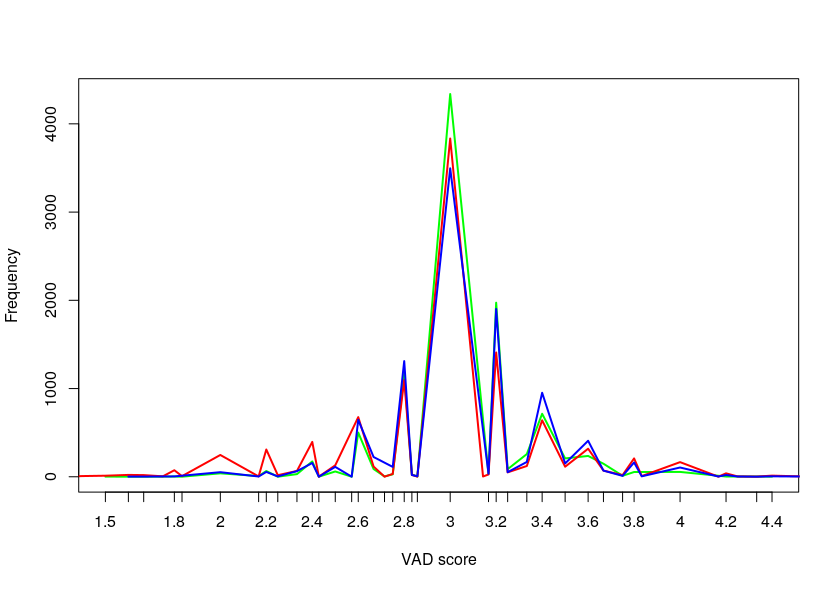
\includegraphics[scale=0.5]{graphs/VADdistribution.png}
\caption{Graph showing data distribution over the Emobank Dataset. R: Valence, B: Arousal, G: Dominance}
\label{dist:vad}
\end{figure}

\section{Problem Formulation}

Coming to a decision to use the VAD structure to analyse the sentiment of text and selecting two valid datasets means that the research questions that were set out can be broken down further.

\subsection{RQ 1}
"How can textual sentiment prediction be optimised?" 
\\ This can be refined into the following: 

\begin{itemize}
    \item Ensuring the input text into the model is best suited to the type of analysis that will be carried out over it. 
    \item Analysing what the existing best text based sentiment prediction methods are, and adapting them for predicting VAD values. 
    \item How to deal with a limited and imbalanced dataset, such as the Emobank dataset.
\end{itemize}

To be able to answer these points in a formal way, we can set the base structure of the sentiment prediction model that will be created as shown in Figure \ref{intial:flow}. 
Text will be taken in in the form of sentences, and output values for the Valence, the Arousal and the Dominance will be produced. The output format of the model for each of these dimensions will be based on how the dataset is processed by the model, as the continuous values for the VAD dimensions will be turned into discrete variables which is looked at in more depth and analysed further.

To deal with input sentences, they will be vectorized so that the model can deal with the data. This is a common way of dealing with text data \cite{towardsDS}, and turns a sentence into a sparse vector over the length of the whole vocabulary, with an integer count for the number of times a word has appeared in the sentence. Finding the best way to deal with the produced vectors will be explored further as part of an investigation into pre-processing the data. 

\begin{figure}[h]
\centering

\includegraphics[scale=0.5]{litImgs/initialFlow.png}
\caption{Diagram showing the flow of data through the sentiment analysis model}
\label{intial:flow}
\end{figure}

\subsection{RQ 2}
"Is using more than 1 dimension to classify emotions useful?"
\\ To refine this question we need to state what we can judge "usefulness" by in this context, and how we can make sure that this is quantified.

To judge whether using more than 1 dimension to is useful, an investigation will be carried out that explores whether applications can be built with the resultant model that utilise the extra information in an effective way. To analyse whether a produced emotional rating is correct, we will also need to have user testing involved, since sentiment is such a subjective concept. The creation of a web application through which a user can accurately judge whether the output is correct provides a platform from which this can be investigated.



\section{Related Work}
\subsection{Sentiment Analysis Tools}

Many existing sentiment analysis tools are tailored towards market research for businesses, so focus on providing opinion mining tools for social media. This means that they focus on extracting the Valence, and the subject that is being discussed. In terms of obtaining an emotion from a piece of text, this binary structure of representing all possible sentiments is very limiting. Emotion can be argued as more than just "Happy" or "Sad", so there is a considerable interest in exploring this further.

There seems to be very little existing work which tries to use semantic analysis to predict more than just the Valence of text, so comparing this to existing work is a challenge. Commercial solutions tend to present their final sentiment analysis models as an API which can be harnessed for general use, and an example of this is Amazon Comprehend.

The Amazon Web Services (AWS) Platform offers Amazon Comprehend \cite{aws} as a sentiment analysis product to customers. This is a Natural Language Processing (NLP) tool that extracts attributes such as a positive or negative Valence, and entities such as locations that are being discussed in an input. When tested with a misleading piece text, it does not predict the sentiment well, as shown in Figure \ref{aws:sentiment}. The sentence used here contains both positive and negative emotions , which is where the structure of representing emotion in one dimension is limiting. This is an example of where using a more complex structure can come into use. 

\begin{figure}[ht]
\centering
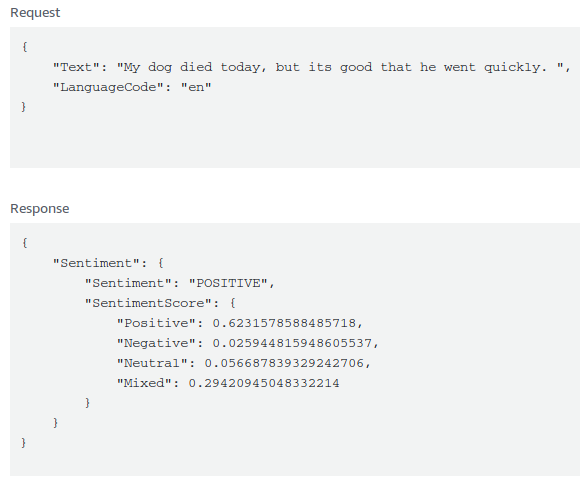
\includegraphics[scale=0.6]{litImgs/comphrendResult.png}
\caption{A display of the input text and incorrect analysis of the sentiment of it by the Amazon Comprehend service}
\label{aws:sentiment}
\end{figure}

\subsubsection{Data Pre-Processing Approaches}

To ensure the input text is in the best format for carrying out sentiment analysis upon, previous work has been analysed to ascertain how this can be optimised.
R. Kim's series on investigating sentiment in Twitter data \cite{towardsDS} has been very influential in this project for inspiring different ways that the data can be pre-processed.
The two main ways that R. Kim's experiment is done is by varying the N-Gram value and number of features supplied to the model.

To preserve the relationship between the words in a sentence, N-grams are very useful since they can help maintain negation of words and helps keep the overall sentiment given in the input sentence better, as shown in Figure \ref{ngrams}. The number of features in this experiment is the $x$ most frequent N-Gram "words" that appear in the dataset.

\begin{figure}[h]
\centering
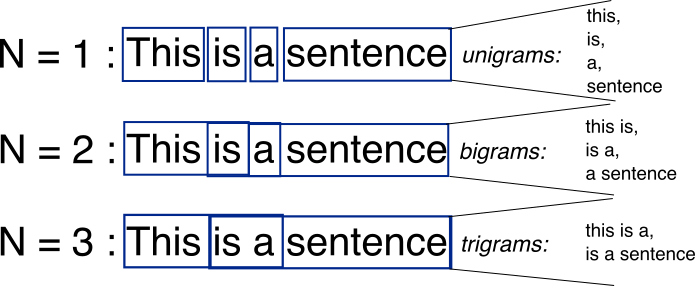
\includegraphics[scale=0.5]{litImgs/ngrams.png}
\caption{Diagram showing the way that the n-grams are created}
\label{ngrams}
\end{figure}

During the experiments put forward by R. Kim, unigrams, bigrams and trigrams are compared and analysed over a feature range of 10000 to 100001. These experiments are done over a totally balanced dataset, with 50\% of the data being classed as having a positive Valence, and the other 50\% with a negative one, and produce results as shown in Figure \ref{towards:DS} that imply that these methods are worth investigating, but can be improved upon.

\begin{figure}[h]
\centering
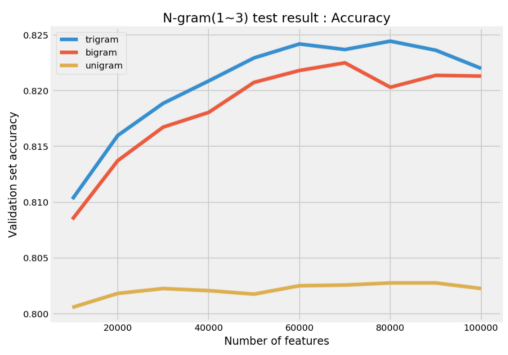
\includegraphics[scale=2.5]{litImgs/towardsDSNgramNFeatures.png}
\caption{Results from R. Kim's investigation over the Sentiment 140 Dataset \cite{go2016sentiment140}}
\label{towards:DS}
\end{figure}

Using these methods, our data flow through the system is now represented in Figure \ref{model:flow}.

\begin{figure}[h]
\centering

\includegraphics[scale=0.5]{litImgs/modelFlow.png}
\caption{Diagram showing inputs and outputs of the model}
\label{model:flow}
\end{figure}


\pagebreak

\subsubsection{Model building approaches}

A common way of creating a semantic analysis tool is to use movie reviews as mentioned before since these already have numeric values attached to them, or Twitter data due to the sheer volume of text available. Since previous sentiment analysis tools have all been done by training over datasets with the Valence values in discrete variables, Positive and Negative, sometimes with a Neutral class as well, the continuous variables given in the Emobank dataset will be bucketed into classes so that similar methods can be applied. An investigation into finding the optimal number of classes to split the data for each VAD dimension into will be carried out.

When analysing the Valence of tweets, using a lexicon based model, as well as implementing machine learning approaches have been used to great effect \cite{kolchyna2015twitter}, and hence these will be the methods investigated in the the creation of a prediction model.

There has been only a little research into using a multi-dimensional VAD structure to investigate sentiment, one paper primarily explores whether using a VAD structure could be used to help identify burnout in software developers \cite{mantyla2016mining}. In this case, a correlation was found between each of the VAD dimensions and issues raised in messages from the developers, meaning that there is an argument for using multiple dimensions to help understand textual data to a greater degree. An issue with this research is that they only used a word based lexicon where each individual word was assigned a value. This loses the context where which each word is being used, and by using N-Grams this issue will be mitigated.

Before exploring machine learning approaches, a lexicon based model will be established. This is using the bag-of-words dataset \cite{wordsData}, where each individual word in the input sentence is looked up in the dataset, assigned a value, then an average can be taken over the input sentence to give a resultant VAD score. This method has been used before to great effect with binary Valence classification, and so investigating it in this case should lead to promising results \cite{kolchyna2015twitter}.

When choosing the machine learning based classifiers to investigate, literature shows that the same few classifiers such as Logistic Regression and Naive Bayes tend to show the best results for analysing textual data \cite{kolchyna2015twitter} \cite{frank2006naive}.

Logistic Regression is popular due to it being linear and scalable for large datasets \cite{towardsDS}. This is the model that will be initially used for comparing data pre-processing results since it is easy to implement and other work has found it to be the best result for their data. 
Other classifiers that have been shown to give positive results for textual analysis tasks are different styles of Bayes classifiers,  which depend slightly on how many classes are being used. Multinomial is the most common for text categorisation problems, so this one will also be of high interest \cite{frank2006naive}. Support Vector Machines (SVM) have also been used in the past for text classification purposes with a positive results, so these will be incorporated as well \cite{joachims1998text}. Previous work tends to avoid using computationally expensive approaches such as K-Nearest Neighbours and Random Forests due to the size of the datasets being used, but since the Emobank dataset is not that large, it is worth investigating those models as well. To compare these models further, we will also take a note of a rough estimate time it take for each classifier to run, to give us an idea of how much computation each needs.

\subsubsection{Over and Undersampling}

Due to the imbalance of data across the Emobank dataset as shown in Figure \ref{dist:vad}, trying to mitigate the effects of this is a challenge that has different ways of being tackled, and one common way of doing this is through oversampling the minority classes in the data to create a more balanced dataset \cite{towardsDS}.

Since manually inputting more data would take more time than is sensible, the most common way to oversample the data that we are given, is through SMOTE (Synthetic Minority Oversampling Technique). This uses a K-Nearest neighbours approach to create synthetic data of the existing minority samples , and has been shown to have positive results with general machine learning tasks but has been known to be problematic with textual data, due to not actually creating synthetic samples which make logical sense. Investigating this method is worthwhile, although the expected results are fairly unknown as it depends heavily on the data in the minority classes. SMOTE tends to be simpler for continuous data \cite{chawla2002smote}, but we are turning the VAD values into discrete classes so this may lead to more difficulty in creating synthetic samples with accurate VAD scores. Since we will also be applying SMOTE to textual data however, where the synthetic text is likely to not make any sense, the issues caused by this should be minimal in comparison. 

There are other popular oversampling techniques that exist as well, for example just randomly re-sampling the minority class, as well as ADASYN (Adaptive Synthetic Sampling) which is a a form of a SMOTE oversampler which works better for classifiers without clear class boundaries, which will also be investigated.

Another, slightly different approach is to undersample the data, removing less important samples from the majority class so that the dataset is more balanced. This in itself can cause issues since the amount of data that can be trained off is reduced, and literature shows that it tends to not have positive results for textual data, but since it can be used in circumstances when there is not enough data in the minority class to create decent synthetic samples in oversampling, it is worth exploring in this case \cite{more2016survey}. There are different methods of undersampling, from randomly removing items from the majority class, to using the NearMiss undersampler, which uses K-Nearest neighbours to select suitable samples to remove. 

The flow of the data can now be represented by Figure \ref{model:finalFlow}.

\begin{figure}[h]
\centering

\includegraphics[scale=0.5]{litImgs/finalmodelflow.png}
\caption{Diagram showing the flow of data through the sentiment analysis model including over/undersampling techniques}
\label{model:finalFlow}
\end{figure}

\subsection{Presenting Results}

Existing sentiment analysis tools either do not do anything with a final model, or use the tool as an API for use in general projects \cite{sentimentAPI}.  

To be able to present in the final model in a way that can be used to analyse whether it is useful, an API will be created from it and a web application that can access the data will be produced to allow for further analysis.

Music is also something  that cannot be easily classified into a binary sentimental structure, so relating the output VAD values of the produced model to songs is something that is worth exploring, where a use can be found to directly apply each of the dimensions.

An existing product that does this is the MoodTape web application, which uses the Valence of input text and relates this to the Valence of a song  \cite{moodtape}. Since, as shown in Listing \ref{spotifyJSON}, much more information can be obtained from individual songs than just the Valence, as shown when requesting song data from the Spotify API, an improvement of this project would be to relate the Dominance and Arousal dimensions to some of the other attributes.
\pagebreak
\begin{lstlisting}[style=leftCode, caption={Some of the attributes of a song obtained through requesting information through the Spotify API},captionpos=b, label={spotifyJSON}]
{
    "danceability": 0.322,
    "energy": 0.0593,
    "key": 1,
    "loudness": -53.057,
    "speechiness": 0.0444,
    "acousticness": 0.908,
    "instrumentalness": 0.708,
    "liveness": 0.121,
    "Valence": 0.0165,
    "tempo": 158.402,
    "time_signature": 4
}
\end{lstlisting}

Using a web UI to present the results that has been done in the MoodTape application, and is probably the simplest way to gather all the data together, and so a web application will be produced to provide a basis to answer RQ \ref{RQ2}.

What we can class as "more useful" as can be quite subjective, and as such discussions will be held with test users about how well they believe the predicted song fits them.
   
\section{Methodology}
 
To ensure RQ \ref{RQ1} is answered, a set of investigations will be carried out to directly answer the points brought up in the Problem Formulation, and by the use of hypothesis tests be able to come to solid conclusions. 

To answer RQ \ref{RQ2}, an exploration into finding the optimal way to present an interface to gather user feedback will be carried out.

\subsection{Data Imbalance}

The initial issue faced when starting to attempt to build a prediction model was how to split the continuous variables supplied by the EmoBank dataset into discrete categories.

The decision to split the data into discrete categories was done since it is easier to utilise classification methods produced by previous work as they tend to use discrete classes like Positive, Neutral and Negative to represent sentiment. The output data for each V,A,D value will be defined as one of a set number of classes, the same number of classes as the input.

To discover the optimal way that the data can be split, the imbalance created over the dataset when the the classes are split in different ways will be analysed and compared. The imbalance over the data should ideally be as low as possible.

\subsection{Hypothesis Tests}

To argue for each of the decisions made when building the final model, a hypothesis test with a 95\% confidence level will be carried out.

Due to the imbalance in the data, a prediction accuracy cannot be used for comparing the models. This is because the majority class dominates \cite{al2015applied}, heavily biasing the accuracy results.

For each investigation,  a confusion matrix is be produced as shown in Table \ref{conmat}, so that proper analysis of the results can be made.

\begin{table}
\centering
\begin{tabular}{|p{3cm}|p{3cm}|p{3cm}|p{3cm}|p{3cm}|}
 \hline
  & \multicolumn{3}{|c|}{Predicted} & \\
 \hline
   Actual & Negative & Neutral & Positive & \\
    \hline
    Negative &  True Negative   &  False Negative  & False Negative & Total Negative \\
    Neutral & False Neutral & True Neutral&  False Neutral & Total Neutral \\
    Positive & False Positive & False Positive &  True Positive & Total Positive \\
    \hline
    & Total Predicted Negative & Total Predicted Neutral & Total Predicted Positive & \\
 \hline
\end{tabular}
\caption{Structure of produced confusion matrices}
\label{conmat}
\end{table}

The F1 score of the prediction model is used in the hypothesis tests. The F1 score for a class is the weighted average of the precision and recall of it, which is defined as follows: 

$$ F1_{Class} = 2 * \frac{Precision_{Class} * Recall_{Class}}{Precision_{Class} + Recall_{Class}} $$

And then the precision and recall values can be calculated as follows, calculated from the confusion matrix given in Table \ref{conmat}.
For example, for the Negative class:

$$ Precision_{Negative} = \frac{\textnormal{True Negative}}{\textnormal{Total Predicted Negative}} $$

$$ Recall_{Negative} = \frac{\textnormal{True Negative}}{\textnormal{Total Negative}} $$

It follows for the other two classes in the same format.

Using this F1 score instead of the accuracy gets rid of the class bias, and in this case it is calculated using the micro-average of the K-Folds. The micro average aggregates the contributions of each class so that any imbalance can be mitigated. The resultant F1 score is given on a scale between 0 and 1, where 1 is perfect prediction.

The hypothesis test that will be performed on the data will be the Wilcoxon Signed-Rank Test, since the comparison between the data will be on two related samples, and the data cannot be assumed to be normally distributed within the folds, meaning that this is the best test to be using in this case \cite{wilcoxon1970critical}.

Each of the experiments will be run with stratified K-Fold validation, with the data from each fold being used for the hypothesis test comparisons, using 10 folds. The folds are stratified so that the representation of each class remains the same in each run, which is needed due to the large data imbalance \cite{kohavi1995study}.

\subsection{Lexicon Analysis}

For the bag-of-words model, we will calculate the confusion matrix and then the F1 score by totalling up the values for each sentence over the Emobank dataset, and then comparing the two results, the calculated values, and the ones given in Emobank sample. The values are calculated by looking up each word in the bag-of-words dataset and creating an average for the sentence.

To get the words from the EmoBank dataset into a state where they are most likely to be found within the lexicon database, some natural language processing needs to be done on the data, using the NLTK \cite{NLTKBook} library to stem the words, returning them to their root form.

For example, the word "Fishing" would be reduced to the word "Fish" after being stemmed. 

As we can see from Figure \ref{lexiconGraph}, the average values for the Arousal are much lower across the bag-of-word dataset than the average values for the Valence or the Dominance, which may have an effect on the output results since the three dimensions in the EmoBank dataset have similar average values as shown in Figure \ref{dist:vad}.


\subsection{Data Pre-processing (N-Gram and Feature selection)}

Following R. Kim's investigations into semantic analysis \cite{towardsDS}, an investigation into optimising the format for the data input is carried out. 

After countvectorizing the text, the number of features and N-Gram values are investigated. The previous investigation only tried N-Gram values ranging up to trigram, but to ensure that this is an optimal result, the experiment will be carried out up to fourgram.

The range of features that was used previously was up to 10,0000 features because the results did not improve after this, but since we are using a different dataset, the number of features tested will be increased until the resultant graph implies that the F1 score does not improve further.

The model used to investigate how the F1 score varies with these inputs will be a Logistic Regression classifier, as this has been shown to give the most promising results in previous work \cite{towardsDS}, and to compare the results in the hypothesis tests we will use the Valence dimension, as previous work uses the Valence of text to build their models and it will be easier to compare to them.

\subsection{Model Selection}

To choose the models to compare, we will take the top models in previous sentiment analysis tools and see which can work best in this situation. 

In R. Kims investigations, Logistic Regression and Linear Support Vector Classification (SVC) were found to be the best so these will be part of the comparison, and we will set Logistic Regression to be used as a base to carry out initial comparisons. 
Other models that will be investigated are Mulitnomial Naive Bayes and Bernoulli Naive Bayes since these are known to perform well with text based tasks \cite{socher2013recursive}, as well as including the computationally expensive models, K-Nearest Neighbours and Random Forests. 

\subsection{Oversampling and Undersampling}

To carry out the investigation of applying the oversampling and undersampling methods, the library functions in the imblearn API are used, which can be used in conjunction with the sklearn methods easily \cite{sklearn}.
Since it is unclear whether these methods will actually improve the model, comparing against the base model that we already have at the point where this investigation is carried out is necessary. As set out in the Related Work, how these methods will perform will depend on how the data is set out into discrete classes.

\subsection{Implementation}

In terms of developing the sentiment analysis tool, using Python is a clear choice due to the number of NLP and machine learning libraries available. The main library that will be utilised is the sklearn library \cite{sklearn}, as it has many in-built machine learning classifiers that can be implemented easily, and there is plenty of documentation to support development with this. 

Using other libraries such as Tensorflow is also applicable in this case,  and they are a powerful tool for building models that utilise neural networks, but in this case using the "off-the-shelf" classifiers given by the sklearn library is all we need.

The simplest solution to provide an interface between the final produced semantic prediction model and the Spotify API, to relate the input text to the music, is to create a web application. The Spotify API is a service which can be used by developers to utilise user and song data within the service \cite{nodeSpotify}, allowing access to a large dataset of music where each song is annotated in with in depth information, such as the information shown in Listing \ref{spotifyJSON}.

The final classification model will be hosted on a very simple python server that takes text as an input, and returns whether it classes the text as Positive, Negative or Neutral for each of the Valence, Arousal or Dominance dimensions, so that predictions can easily be made from a web application using HTTP requests. The final solution, as shown in Figure \ref{implementationLayout}, will consist of three distinct hosted solutions, two of which access the API hosted by Spotify to access song data.

The UI has been chosen to be built in Angular.js and the music API with Node.js due to prior development knowledge, and hence ease of prototyping. 
To ensure that any resultant song given back was one that the user could relate to, the final song is taken from a selection of the users recent top songs, which they allow the application access to through the authentication process.
The music API, built in Node.js is influenced by the structure of existing Spotify API projects \cite{moodtape}, and is built mostly using the Node package spotify-web-api-node \cite{nodeSpotify}.

\begin{figure}[ht]
\caption{General layout of how the web application should be structured.}
\centering
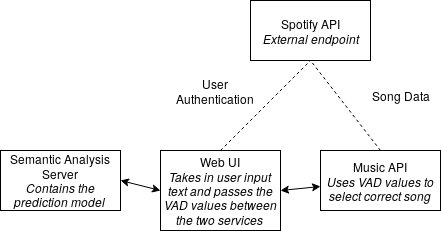
\includegraphics[scale=0.6]{litImgs/interfaceLayout.png}
\label{implementationLayout}
\end{figure}

Choosing how to relate the VAD values to the data returned for the songs is relatively arbitrary, and something that if there was more time could be investigated further. Since the song data returns a Valence value, it is obvious to map those two attributes together, and it was chosen to map the Arousal to the "Energy" attribute, and the Dominance to the "Danceability", but this is something that can be improved upon.

The main goal of the implementation is to attempt to relate an emotion in text, which is subjective, to a song since that is also subjective. To help clarify whether the model is appropriate, the closest Ekman's emotion as given in Table \ref{ekmansTable} will be calculated and conveyed back to a test user for discussion, as well as a calculated song. This emotion will not be exact due to the choice of putting the variables into discrete classes and the closeness of some of the emotions as shown in Figure \ref{ekmans:graph}, but the result should help the users assess whether the given prediction is correct. The choice not to show the users the direct VAD values is made so that the users do not need an explanation of the structure to understand the emotion behind it. The Ekmans emotion will be calculated by finding the shortest distance between the calculated point and the values in Table \ref{ekmansTable}.

\begin{figure}[ht]
\centering
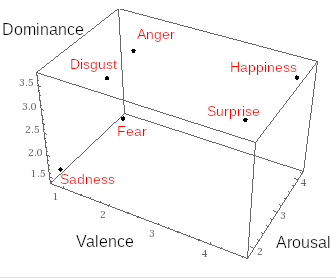
\includegraphics[scale=2]{litImgs/Ekmans3d.png}
\caption{3D plot of the figures given in Table \ref{ekmansTable}}
\label{ekmans:graph}
\end{figure}


To ensure RQ \ref{RQ2} is answered, the following questions will be set to the test users:

\begin{itemize}
    \item Do you believe the output song relates well to the text that you have input? Why?
    \item Do you think this (calcuated Ekmans) emotion fits the text and the song well?
\end{itemize}
\section{Results}
\subsection{Data Imbalance}
An initial look at the data shows that there is a large number of sentences represented with values a neutral area, and very few representing the extreme cases, as shown in Figure \ref{dist:vad}.

The simplest way to initially categorise the data is to round to the nearest whole number, but as shown in Figure \ref{dist:5cat}, the extreme classes are not well represented, and would prove very difficult to train a model off. Having 5 discrete classes for each dimension also provides more detail than is probably necessary for the task at hand, so can be simplified

Splitting each dimension up into positive or negative values is also is an option, allowing an easier comparison to other work which generally does this. The issue here is that the data imbalance is still very great, particularly with the Arousal and Dominance dimensions, as shown in Figure \ref{dist:bin}.

\begin{figure}[h]
\centering
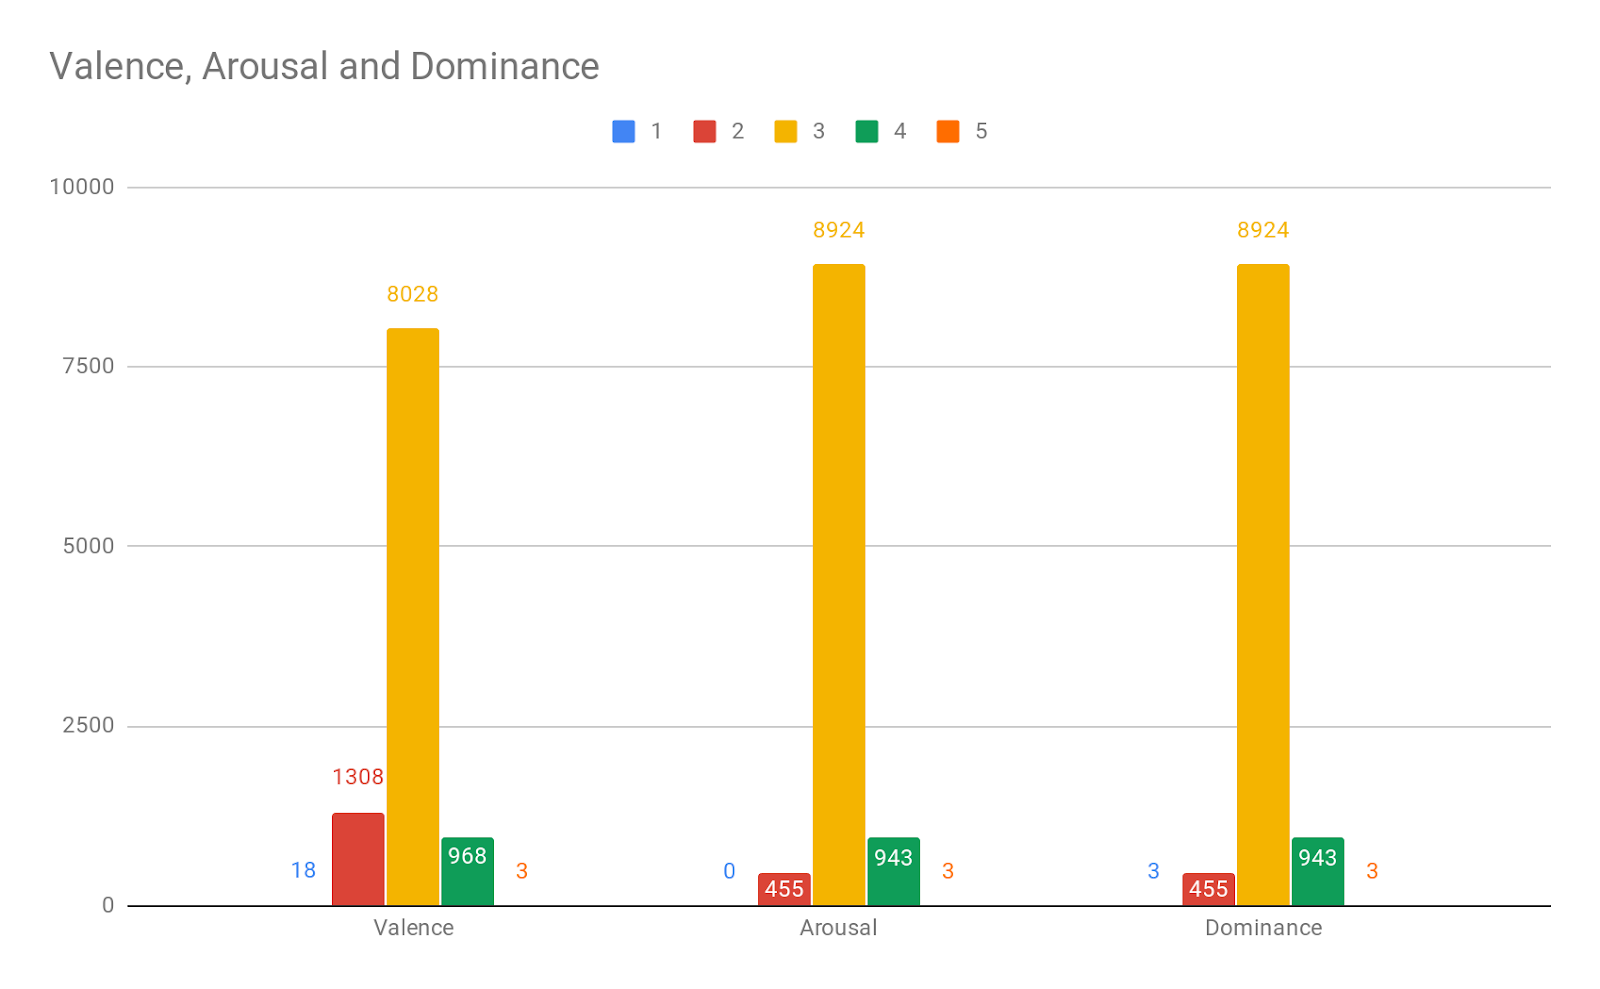
\includegraphics[scale=0.3]{graphs/5catDist.png}
\caption{Graph showing data distribution when split into five classes, where 1 is negative and 5 is positive}
\label{dist:5cat}
\end{figure}

\begin{figure}[ht]
\centering
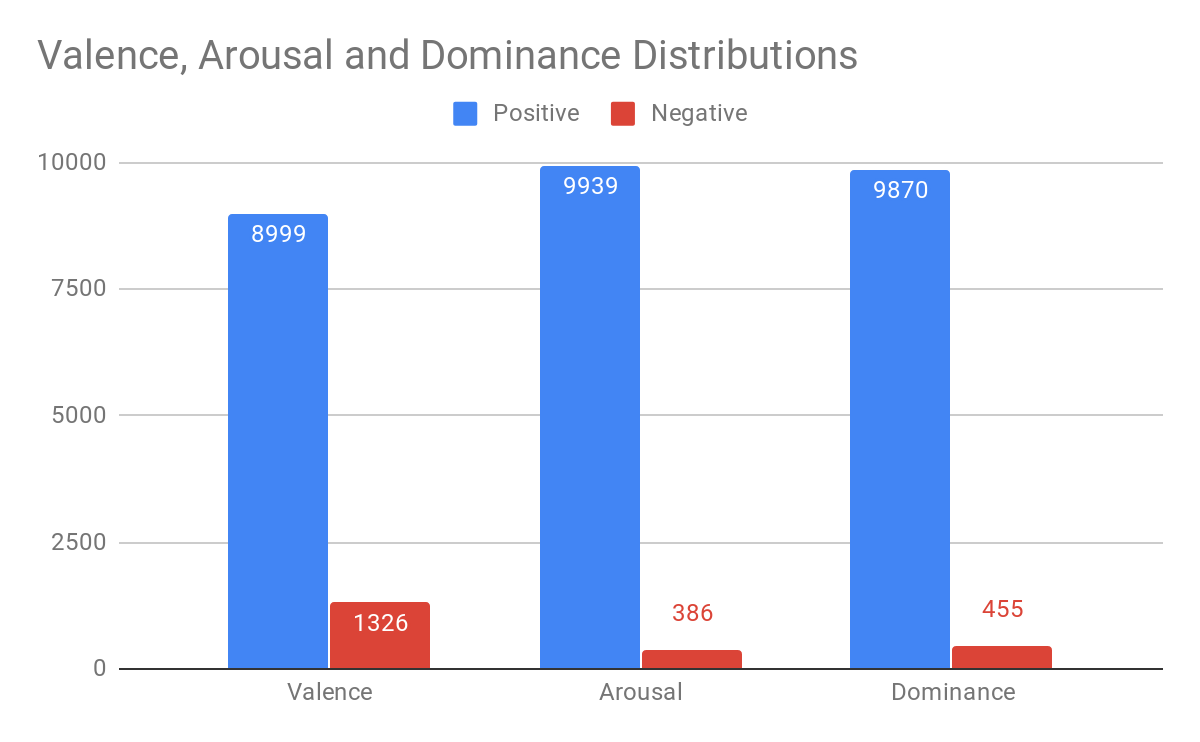
\includegraphics[scale=0.3]{graphs/binaryDist.png}
\caption{Graph showing data distribution when split into binary positive and negative classes}
\label{dist:bin}
\end{figure}
\pagebreak
A middle ground can be found when splitting the data into positive, neutral and negative classes, as even though there is still a data imbalance there, it is less severe, shown in Figure \ref{dist:tri}, and as such will be used as the structure moving forward.

\begin{figure}[H]
\centering
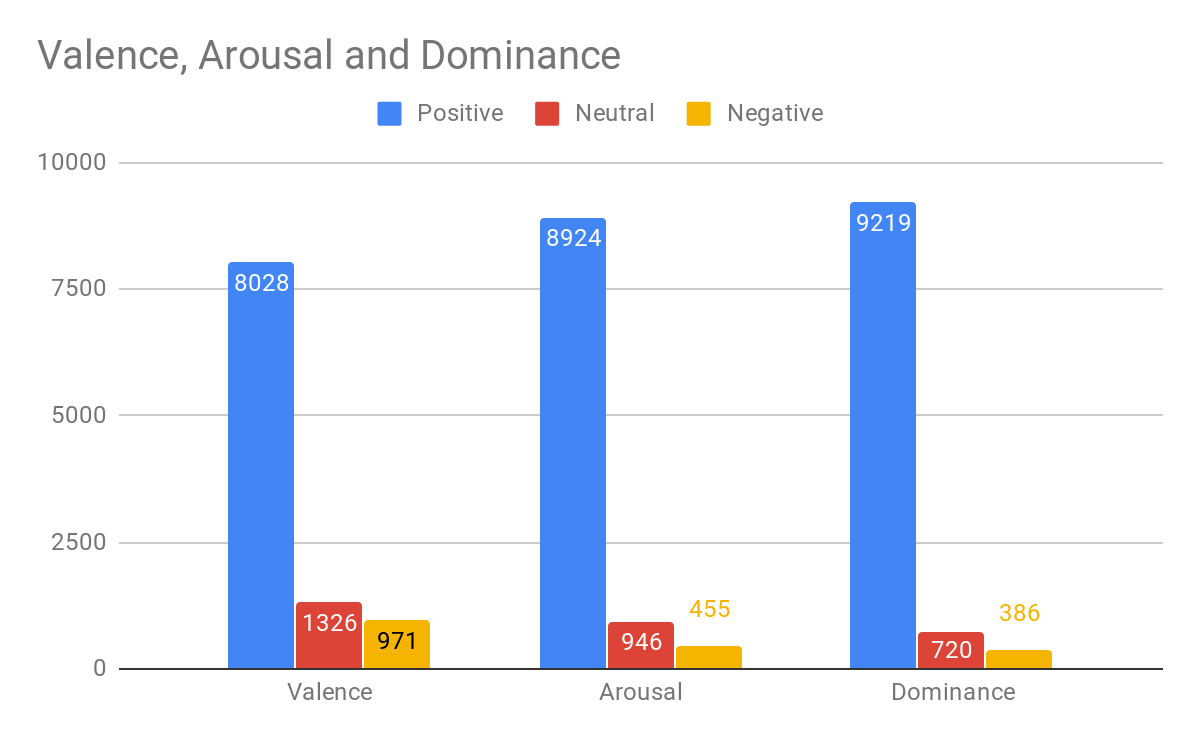
\includegraphics[scale=0.35]{graphs/nonBinaryDist.png}
\caption{Graph showing data distribution when split into positive, neutral negative classes}
\label{dist:tri}
\end{figure}

\subsection{Lexicon Analysis}

After carrying out an investigation into using the bag-of-words dataset with the Emobank dataset for predictions, the following results are obtained:

\begin{table}
\centering
\caption{F1 scores for the 3 dimensions for the bag-of-words model}
\begin{tabular}{ |p{3cm}|p{3cm}|}
 \hline
  Dimension & F1 Score \\
 \hline
  Valence & 0.72\\
  Arousal & 0.08 \\
  Dominance & 0.80\\
 \hline
\end{tabular}
\label{lexicon:f1}
\end{table}

We can see in Table \ref{lexicon:f1} that for the Valence and Dominance dimensions, using lexicon analysis as a form of prediction performs quite well, and whether these scores can be further improved with machine learning methods will be interesting.

To explore why the Arousal dimension performs so badly, we can take a closer look at the generated confusion matrix, as shown in Table \ref{lexicon:a:conmat}. As we can see, most of the neutral data was predicted to be negative, which is definitely influenced by the trend in the bag-of-words dataset, where the average values for the Arousal are quite low. There are also no correctly predicted values in the positive class, which also contributes to the extremely low F1 score.

\begin{table}
\centering
\caption{Confusion matrix for Arousal}
\begin{tabular}{ |p{3cm}|p{3cm}|p{3cm}|p{3cm}| }
 \hline
  & \multicolumn{3}{|c|}{Predicted} \\
 \hline
   Actual & Negative & Neutral & Positive \\
    \hline
    Negative &  313   &  10  & 0 \\
    Neutral & 7001 & 384 &  3 \\
    Positive & 656 & 83 &  0 \\
 \hline
\end{tabular}
\label{lexicon:a:conmat}
\end{table}


It is also worth noting that the values in Table \ref{lexicon:a:conmat} do not cover the whole dataset either, due to instances when all of the words in the EmoBank sample cannot be found within the lexicon dataset. In this case there are around 1,500 sentences for which a VAD value could not be calculated, showing that this bag-of-words based method is far from optimal since all of the data cannot be analysed.

\subsection{Data Pre-Processing}

This experiment is the investigation into changing the number of features and size of N-Gram words with the Logistic Regression classifier. The Valence dimension is used here for comparison of results.

\begin{figure}[h]
\centering
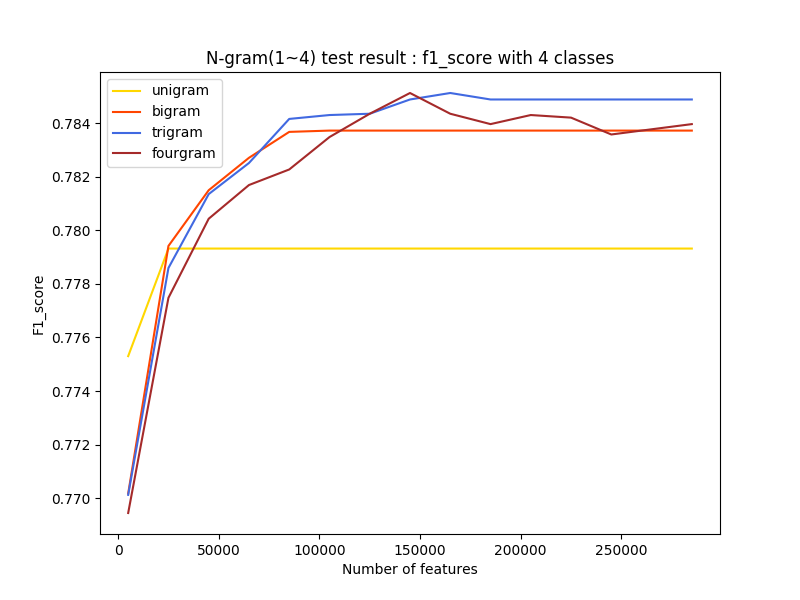
\includegraphics[scale=0.7]{graphs/nGramBinaryGraph300000.png}
\caption{Experimental Results for varying the number of features and values for N-Gram words}
\label{ngramGraph}
\end{figure}

As shown in Figure \ref{ngramGraph}, the F1 score improves as the N-Gram value increases up to a point, and the score also increases as the number of features does. An explanation of why the values for fourgram are generally less than for trigram, could be because the dataset is not that large and therefore predictions are less accurate as the relationships between the words cannot be properly established, so for our purposes we can leave out fourgram. It requires a significantly higher amount of processing time, as shown in Table \ref{ngram:time}. The values in Table \ref{ngram:time} are estimates calculated just to show the scale differences between the variables, and would vary depending on the amount of processing power availible.

\begin{table}
\centering
\caption{Approximate Computation time for each N-Gram value.}
\begin{tabular}{ |p{3cm}|p{3cm}|}
 \hline
  N-Gram selection & Time (s) \\
 \hline
  unigram & 71\\
  bigram & 241\\
  trigram & 406\\
  fourgram & 1105 \\
 \hline
\end{tabular}
\label{ngram:time}
\end{table}
\pagebreak

\subsubsection{Hypothesis Tests}

Using the trigram values to compare, as the graph shows that this gives the highest results, the hypothesis test shows that the F1 score still increases after 65,000 features as shown below:

$$ H_0:  \textnormal{F1 score at 65,000 features is the same than at 165,000 features (the peak on the graph)}$$

$$ H_a: \textnormal{F1 score at 65,000 features is less than at 165,000 features} $$


Using the Wilcoxon rank sum test with 95\% confidence interval p = 0.02 so reject $H_0$.
\\But the score for F1 does not increase significantly after 85,000, which is shown as follows:

$$ H_0:  \textnormal{F1 score at 85,000 features is the same than at 165,000 features}$$

$$ H_a: \textnormal{F1 score at 85,000 features is less than at 165,000 features} $$

Using the Wilcoxon rank sum test with 95\% confidence interval p = 0.08 so reject $H_a$.
\\We can conclude that the optimal number of features to use in the model is 85,000, since we reject the alternate hypothesis when using a hypothesis test with a 95\% accuracy if the p-value is greater than 0.05. This number of features will be used in the rest of the investigations as to maximise the score of the resultant model. 

Using this value of 85,000 features, we can compare unigram and bigram results in the following test:

$$ H_0: \textnormal{F1 score of unigram and bigram is the same at 85,000 features} $$
$$ H_a: \textnormal{F1 score of unigram is less than bigram at 85,000 features} $$

Using the Wilcoxon rank sum test with 95\% confidence interval, p = 0.01 so reject $H_0$ and accept the alternate hypothesis.
\\To then check bigram is the optimal, we check the F1 score does not significantly increase at 85,000 features for trigram results, so we carry out the following test:

$$ H_0: \textnormal{F1 score of bigram and trigram is the same at 85,000 features} $$
$$ H_a: \textnormal{F1 score of bigram is less than trigram at 85,000 features} $$

Using the Wilcoxon rank sum test with 95\% confidence interval p = 0.10 so reject $H_a$.
\\ So we can conclude using bigrams is optimal for processing the data for inputting into the model.
The R scripts for running these tests are referenced in Appendix \ref{appendix:hypothesis}.

\subsection{Model Selection}

This experiment is the investigation into changing classification model with 85,000 bigram features. The Valence dimension is used here for comparison of results.

\begin{figure}[h]
\centering
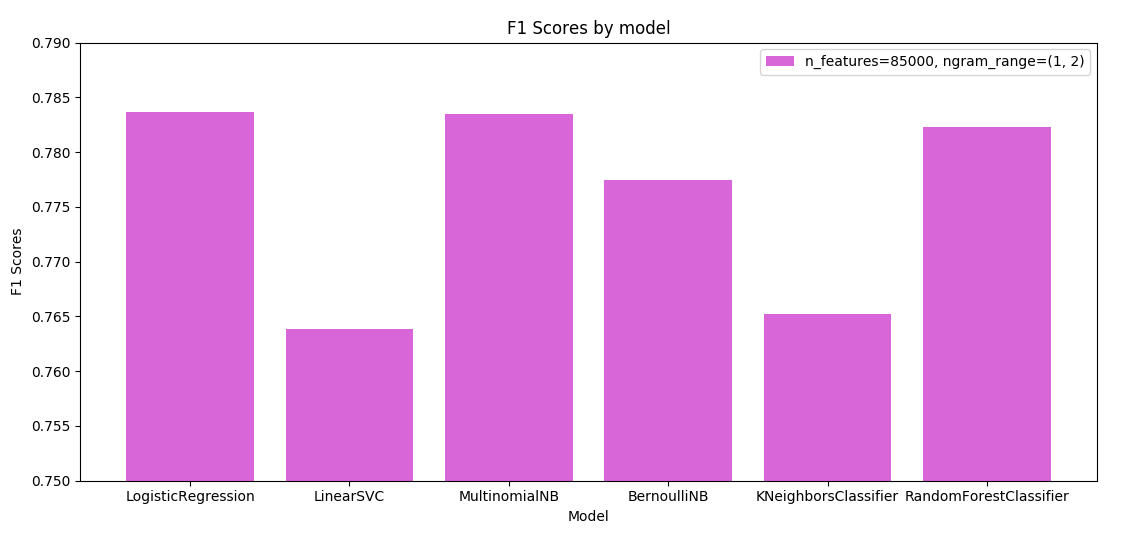
\includegraphics[scale=0.5]{graphs/models.png}
\caption{Graph showing the different F1 scores for varying types of classifier}
\label{model:graph}
\end{figure}

The inbuilt models in the sklearn package with default settings were used for initial comparison, and as we can see from Figure \ref{model:graph} the difference between the models is very slight, with the F1 scores all within a 3\% range. Since each of the models compared are all using their default settings, more work could be done to optimise them further in the future, but just to argue for choosing the best default classifier, the following hypothesis test is run.

\subsubsection{Hypothesis Tests}

We can see that out of the three top models, two of the classifiers that were expected to perform well, Logistic Regression and Multinomial Naive Bayes do so, as well as the Random Forest Classifier. We can prove by hypothesis tests with 95\% confidence interval for a two sided Wilcoxon rank sum test that these three can all be classed as the same, given in Appendix \ref{appendix:hypothesis} To further compare these three models then, we can look at how long it takes for each fold to train and test each model.

\begin{table}
\centering
\caption{F1 scores for the 3 dimensions for machine learning classifier}
\begin{tabular}{ |p{3cm}|p{3cm}|}
 \hline
  Classifier & Average time per fold (s)\\
 \hline
  Logistic Regression & 1.80\\
  Multinomial Naive Bayes & 0.51 \\
  Random Forest & 3.04\\
 \hline
\end{tabular}
\label{model:times}
\end{table}

We can see from Table \ref{model:times} that the Multinomial Naive Bayes Classifier takes a much shorter time to run, so we can select this as the optimal classifier to use.

\subsection{Sampling methods}

This experiment is the investigation into changing the sampling method with the Multinomial Naive Bayes classifier with 85,000 bigram features. The Valence dimension is used here for comparison of results.

We can see from the results from the investigation shown in  Figure \ref{oversamplegraph}, using any of the oversampling methods decreases the F1 score. 

\begin{figure}[h]
\centering
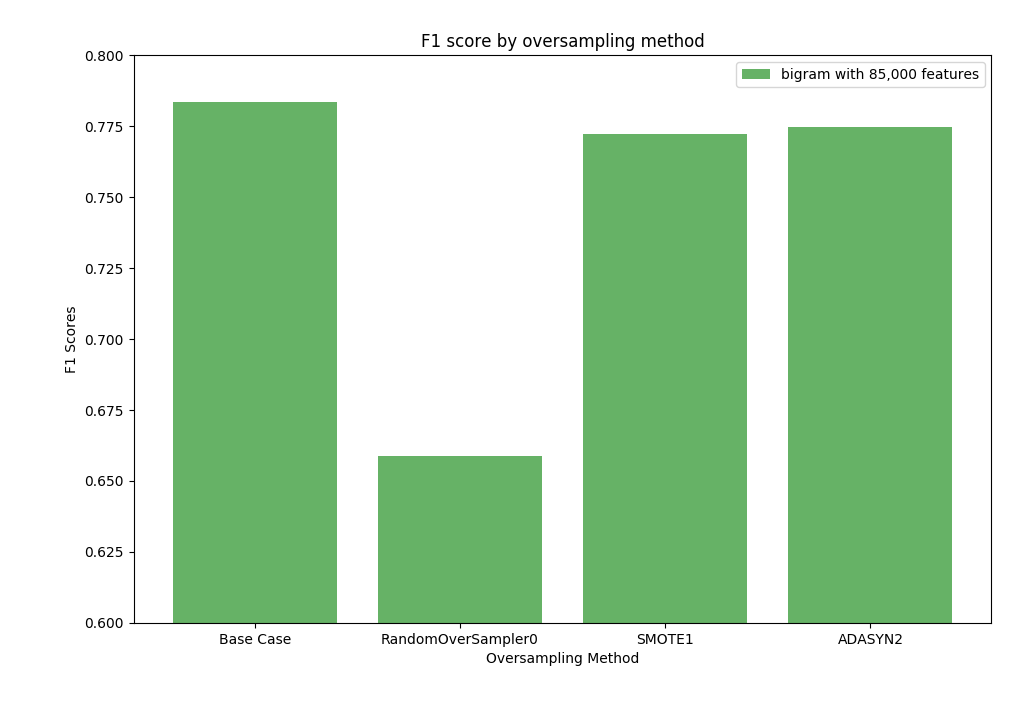
\includegraphics[scale=0.5]{graphs/OversampleNB.png}
\caption{Graph showing the F1 score for different oversampling methods}
\label{oversamplegraph}
\end{figure}

An explanation as to why this is happening is most likely a combination of using textual data, which is known to cause issues with oversampling methods, and the severity of the imbalance in the data. In the Valence class, which is the one we are analysing at this point, the samples in the negative make up less than 10\% of the overall data and therefore many of the synthetic samples that are created will not make grammatical sense and be of poor quality. 

To ensure that the base case is higher than the second highest result, the ADASYN sampler, we run a hypothesis test as follows:

$$ H_0: \textnormal{F1 score of the base case and ADASYN is the same} $$
$$ H_a: \textnormal{F1 score of the base case is greater than ADASYN} $$

Using the Wilcoxon rank sum test with 95\% confidence interval p = 8.98E-5 so reject $H_0$. \\ So we can conclude that using no oversampling methods leads to the highest F1 score.

\begin{figure}[h]
\centering
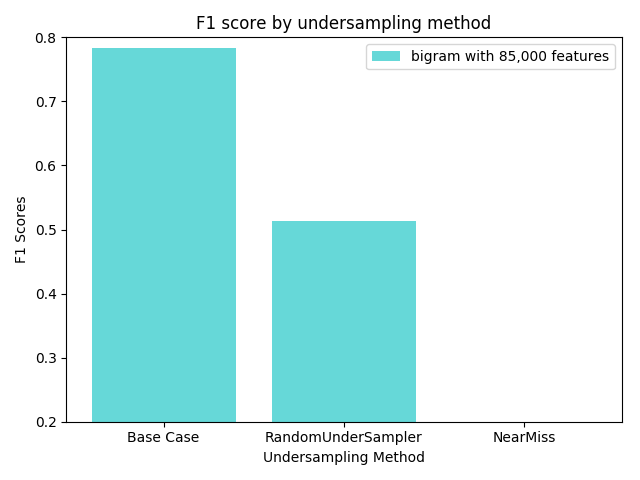
\includegraphics[scale=0.6]{graphs/undersampleNB.png}
\caption{Graph showing the F1 score for different undersampling methods}
\label{undersamplegraph}
\end{figure}

The undersampling methods were known to not give promising results, but due to the issues with oversampling over such a large class imbalance, briefly investigating this was something that could potentially have worked, but as the experimental results shown in Figure \ref{undersamplegraph}, they all made the model perform significantly worse or did not work at all and hence can be disregarded. The near miss undersampling methods did not work as it could not maintain the quality of data while reducing the majority classes to the size of the minority classes, the minority classes were just too small.


\pagebreak

\subsection{Final Model}
\label{finalModelSection}
The final model that was produced then had the following characteristics: 

\begin{itemize}
    \item The data was formatted into bigram "words".
    \item The most frequent 85,000 bigrams were used as input features.
    \item The classification model is Multinomial Naive Bayes.
    \item No oversampling or undersampling techniques were applied.
\end{itemize}

This results in a model that has the F1 scores for the prediction of each dimension shown in Table \ref{ML:f1}.

\begin{table}
\centering
\caption{F1 scores for the 3 dimensions for machine learning model}
\begin{tabular}{ |p{3cm}|p{3cm}|}
 \hline
  Dimension & F1 Score \\
 \hline
  Valence & 0.78\\
  Arousal & 0.86 \\
  Dominance & 0.89\\
 \hline
 Average & 0.843\\
 \hline
\end{tabular}
\label{ML:f1}
\end{table}

\pagebreak

\subsection{Implementation}

A decision was made to not show the user the VAD values, and just the result song to begin with so that their response about the returned song was not affected. After the users reaction to the response song has been assessed, the calculated Ekmans emotion can be shown.

\begin{figure}[ht]
\centering
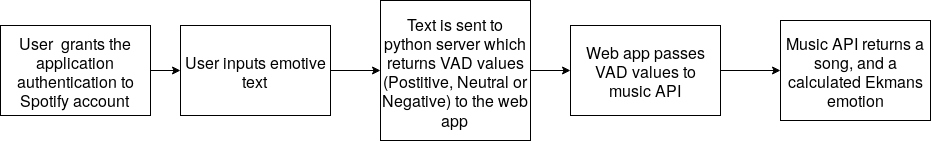
\includegraphics[scale=0.5]{litImgs/interfaceFlow.png}
\caption{User activity through the application}
\label{implementationFlow}
\end{figure}

\begin{figure}[ht]
\centering
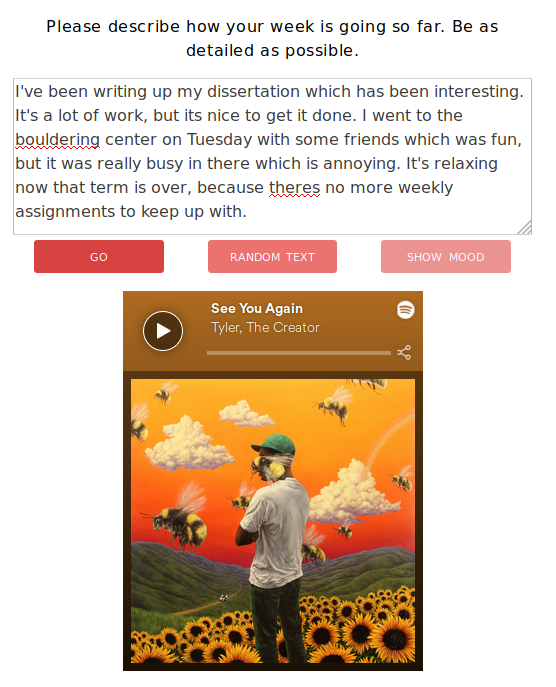
\includegraphics[scale=0.4]{implementation/tamara.png}
\caption{Layout of main UI page}
\label{UIlayout}
\end{figure}

Getting an F1 score of 0.84 on the model is a reasonable result, but testing whether users believe that the model is accurately predicting their emotion is something that needs to be assessed. A screen shot of the produced UI is shown in Figure \ref{UIlayout}.
\pagebreak

\subsection{User Feedback}
Using the built web application we are able gain feedback from test users, asking them to input their own text and access their own Spotify data through the application to obtain a result. 
Out of the five different people that the program was tested with, 3 concluded that the song did match their emotion and 2 did not. This is a very small focus group, and for a more detailed analysis more feedback needs to be gathered, but for the purpose of gaining insight into whether the system is appropriate for answering the research question, an initial idea can be obtained.

All but 2 of the tests gave the result Ekman's emotion back as "Surprise", and the other two came back with "Disgust" which was incorrect every time. An explanation for these results would be because of the way that the data has been split up into discrete classes the 3D distance between the points.

Two users with conflicting opinions on how useful and accurate the implementation is, is set out in more detail as follows:


\subsubsection{User A}

\begin{figure}[h]
\centering
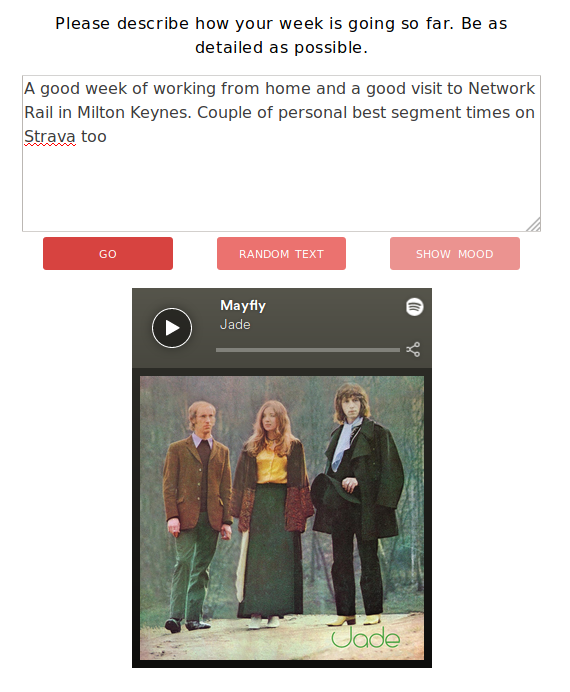
\includegraphics[scale=0.4]{implementation/malc-user.png}
\caption{User A: input and output}
\label{user:1}
\end{figure}

The first user concluded that the song matched what they had input, stating that it was upbeat and had "positive vibes". They did suggest that it would be nice to see how the song was calculated in more detail however. The calculated Ekman's emotion in this case was "Surprise", which was decided was incorrect, particularly when knowing that "Happy" was one of the options that could have been selected. The values for this user are shown in Table \ref{user:1values} and Figure \ref{user:1}.

\begin{table}[h]
\centering
\caption{User A: output values}
\begin{tabular}{|l|l|}
\hline
 Valence &  0.7\\
 Arousal &  0.6\\
 Domiance &  0.5\\
 Ekman's Emotion &  Surprise\\ \hline
\end{tabular}
\label{user:1values}
\end{table}

\pagebreak

\subsubsection{User B}

\begin{figure}[h]
\centering
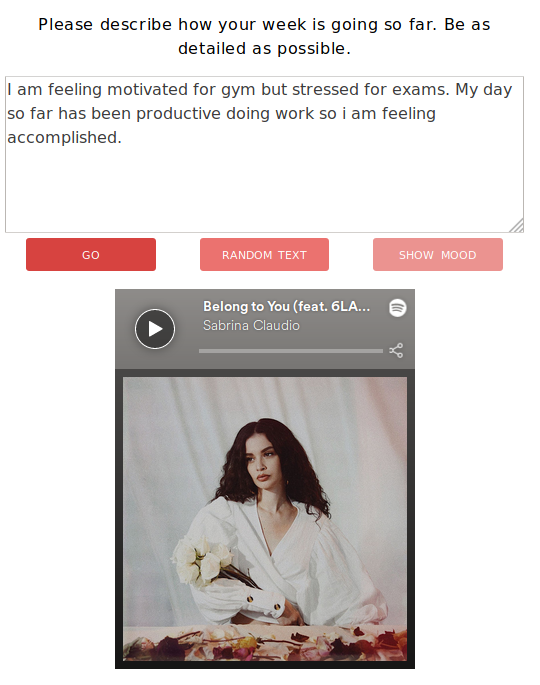
\includegraphics[scale=0.4]{implementation/jana.png}
\caption{User B: input and output}
\label{user:2}
\end{figure}

The second user concluded that the song did not match their mood, since its a very relaxed song, but they did mention that they've been listening to a lot of relaxing music recently. Other reasons why the song did not fit were also discussed, such as words such as "exams" and "work" potentially having an effect on the result. Looking more at the song data behind why this result would have been incorrect, the data Spotify allocated to the song rates it with a high danceability of 0.6, although User 2 disagrees with this. An explanation for this result may be that the Spotify data is not the most accurate, but this is is quite subjective.

\begin{table}[h]
\centering
\caption{User A: output values}
\begin{tabular}{|l|l|}
\hline
 Valence &  0.6\\
 Arousal &  0.6\\
 Domiance &  0.5\\
 Ekman's Emotion &  Surprise\\ \hline
\end{tabular}
\label{user:2values}
\end{table}

\section{Discussion} 
\subsection{RQ 1: How can textual sentiment prediction be optimised?}

Two main methods of predicting the sentiment of input text have been analysed, using a bag-of-words method, and using machine learning approaches.

The lexicon based bag-of-words is based entirely on having an appropriate dataset to rank the words, since as Table \ref{lexicon:f1} shows, having rated VAD scores which follow a certain structure is key to obtaining good results. Dimensions like the Dominance and Arousal of a piece of text can be very subjective, and vary depending on what basis the dataset is judging the scores on.

The decision to use the machine learning based model for the implementation is due to having overall more stable F1 scores for each dimension, but this is only due the model having trained and tested over similar data, from the same dataset.

The use of pre-processing the data, choosing an the best classification model, and selecting appropriate sampling methods lead to the final model established in Section \ref{finalModelSection},  resulting in the highest F1 score we can obtain by trialling these methods. To answer RQ \ref{RQ1}, we can argue that out of the investigations that have been addressed, our conclusions for each of these findings can be decided as optimal, however more work can be done to explore whether the F1 score, and with it the optimality of the prediction model can be increased further.

One point which has not been addressed by this investigation is that the VAD values for each sentence are related to one another. This can be shown by the mosaic plot of the data in Figure \ref{mosaic:emo}, where we can see that the majority of the data is taken up by samples which are neutral in all three dimensions, that is, if the prediction over a sentence returns that it has neutral Valence and Arousal, then it is much more likely to have a neutral Dominance. Figure \ref{mosaic:emo} also displays the Pearson residuals for the data, which shows that for many of the classes that contain Neutral values, particularly neutral Arousal there are a lot less samples than expected when a Pearson $\chi^2$ test is performed \cite{zeileis2007residual}. This test is performed against a null hypothesis that the distribution of values are independent, and in this case it rejects this null hypothesis with a p-value of 2.22E-16.
\begin{figure}[ht]
\centering
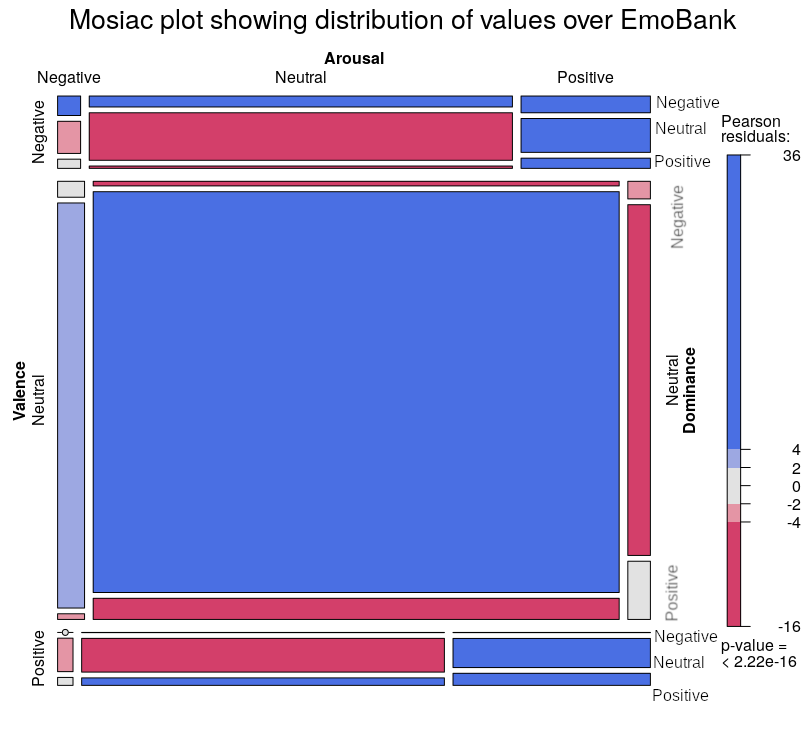
\includegraphics[scale=0.7]{graphs/mosaic_new.png}
\caption{Emobank data distribution with relationships. The Pearson residuals are the deviation from the expected frequency by a Pearson $\chi^2$ Test \cite{pearson1900x}}
\label{mosaic:emo}
\end{figure}

Because of this, a small extension investigation was done using the existing model setup as given in Section \ref{finalModelSection} to train a model to each predict a V, A, D value, given the other two as inputs, as shown in Figure \ref{model:adjust}. Since these adjustment models do not take in the input sentence, the number of feature selection and N-gram values were not needed.

\begin{figure}[ht]
\centering

\includegraphics[scale=0.6]{implementation/adjustModel.png}
\caption{Diagram showing inputs and outputs for the valence prediction model}
\label{model:adjust}
\end{figure}

These models have good F1 scores compared to the model with the sentence data, and more investigation needs to be done on how to incorporate these adjustment models into the final result. 

\begin{table}[h]
\centering
\caption{F1 scores for adjustment models}
\begin{tabular}{|l|l|}
\hline
Model & F1 Score \\ \hline
 Valence Prediction &  0.778\\
 Arousal Prediction &  0.864\\
 Dominance Prediction &  0.893\\
 \hline
\end{tabular}
\label{f1:adj}
\end{table}

\subsection{RQ 2: Is using more than 1 dimension to classify emotions useful?}

Analysing something like insight into an emotion is very subjective, and finding a good way to evaluate this has been difficult. With 60\% of the five test users agreeing with the sentiment behind the output song, it could be said that there is reason to believe that the model produces accurate results. 

Something that has an effect on the calculated song is that it is chosen from the users recent frequent listening history.
What can be done with the Spotify API is to give a time frame from which the pool of top song can be chosen, such as you can choose to only return the top artists from the last week. When the posed question is inquiring into how your week has been going, choosing only the top songs from the past week are much more likely to be related to the users mood from that week. How this affects the output and the users feedback to the song is something that requires more investigation. 

By relating the VAD values to the Spotify data, we can show that applications for using more than 1 dimension can be found since they can be related over more attributes, hence making a multidimensional structure for representing emotion a viable option. Using the responses from this investigation, we can conclude that there is evidence to suggest that RQ \ref{RQ2} can be answered positively, and that useful ways of using a multidimensional sentiment representation structure exist.





\section{Conclusion}

From a personal perspective this project has been thoroughly enjoyable. I had almost no machine learning knowledge before starting, and I have learned more than I had anticipated. Being able to apply new techniques to tools that I was already familiar with has been has been an accomplishment, and I am happy with the final product that has been produced. 

Things that I would do differently now would be to formalise the research questions at an earlier point so that less time was spent exploring things which ended up being unnecessary. I'd have also liked to have spent more time getting to know the data, so that the dependency between the classes could have been investigated further. 

Keeping the VAD values in their original continuous form is also something that would be interesting to explore, and comparing results formed from an investigation into this, to the model used in this project would offer more insight into how the Emobank dataset can be utilised.

Exploring ways in which an emotion can be represented, and using them to the greatest effect has been explored in this project. Future investigation of sentiment representation and analysis can be done with a better understanding by using what has been set out in this report, and more work can be done to attempt to quantify something as seemingly unquantifiable as a human emotion.

\pagebreak


\begin{appendices}

\section{Hypothesis Test Results}
\label{appendix:hypothesis}
The R Script for running the relevant hypothesis test over the data can be found at the following locations:
\begin{center}

% \begin{table}[h]
\begin{tabular}{|l|l|}
\hline
 Test &  Location\\ \hline
 Number of features &  statisticalAnalysis/featureSelection.R\\
 Model Selection &  statisticalAnalysis/modelSelection.R\\
 Sampling Tests &  statisticalAnalysis/overUnder.R\\ \hline
\end{tabular}
% \end{table}
\end{center}

\section{Project File Structure}

The postman layout for all the HTTP requests, with example responses can be found at:
\\ https://documenter.getpostman.com/view/5563343/S1EJXgL9
\\ 
VERSIONS USED: 
\begin{itemize}
    \item Python 3.6
    \item Node  8.10
\end{itemize}

\subsection{Diss}
Contains dissertation .tex files and graphs

\subsection{UI}
Contains UI for running the web application.  To run, Node.js and Angular.js will need to be installed.
To start, navigate into directory and run "npm start", this will automatically install dependencies as well.
This runs on port 8000.
UI Design files are in the ./app directory.

\subsection{Sentiment Analysis}

The final files for carrying out the investigations are in the main directory:

\begin{itemize}
    \item dataProcess.py - Formats each datasets with correct labels and for putting the variables into discrete categories
    \item preProcessingandModel.py - Investigating N-Gram / Number of features / Model
    \item overUnderTest.py - Investigating sampling methods
    \item finalModel.py - Contains a copy of the final model
    \item adjustModel.py  - Contains the adjustment model for dealing with the dependencies between the variables.
    \item bagOfWords.py - Runs the lexicon analysis investigation
    \item ./data -  contains the datasets and output statistics for the hypothesis tests
    \item ./FinalGraphs -  contains the output graphs from the investigations
    \item ./oldFiles - contains initial trials into setting up the investigations.
\end{itemize}


\subsection{Sentiment Python Server}

\begin{itemize}
    \item train.py
    \item server.py
\end{itemize}
train.py contains an instance of the final model as set out by the Sentiment Analysis directory finalModel.py and  hosts it on a very simple python server so that it can be accessed by the web app. 
To run the server, navigate into the directory and run "python server.py". Runs on port 8090.

\subsection{Spotify Data}
To start, navigate into directory and run "npm start", this will automatically install dependencies as well.  This will only run if the secrets.js file is accessible. Runs on port 8080.

\subsection{Statistical Analysis}
Contains the R files for running the hypothesis tests set out.

\section{Project Log}

\textbf{October}
\begin{itemize}
    \item Building project proposal
\end{itemize}
\\
\textbf{November / December}
\begin{itemize}
    \item Literature review
    \item Trialling different ways of splitting the EmoBank dataset up
    \item Count vectorizing the data
    \item Getting familiar with sklearn library using inbuilt Bayes classifier
\end{itemize}
\\
\textbf{January}
\begin{itemize}
    \item Data visualisation
    \item Investigate pre-processing
    \item Introduce different ML methods
    \item Use lexicon analysis dataset for prediction
\end{itemize}
\\
\textbf{February}
\begin{itemize}
    \item Introduce K-Fold validation & Stratified shuffle splits
    \item Introduce oversampling to tackle class imbalance
    \item F1 score comparisons
    \item Begin to build implementation and web application
\end{itemize}
\\
\textbf{March}
\begin{itemize}
    \item Finish implementation
    \item Ensure calculated graphs are in the correct format
    \item Prepare for presentation and begin dissertation
    \item Run hypothesis tests
\end{itemize}
\\
\textbf{April}
\begin{itemize}
    \item Finish dissertation
\end{itemize}
\end{appendices}






\bibliographystyle{unsrtnat}
\bibliography{ref,lit}


\end{document}
